\chapter{Grammar and Induction}

\begin{quote}
``... small number
of symbols and their grammar are enough to capture the huge
variety of equations...''
\end{quote}

Ask yourself how you know what to do when  
substituting for $x\defeq 7$ in $x(x+3)^{2}$.
(Using $\defeq$ indicates an assignment, not an equality variable.)
Whether obvious or not, we start by parsing the grammar.  We can make this 
visual with a \emph{parse tree}.
\begin{center}
    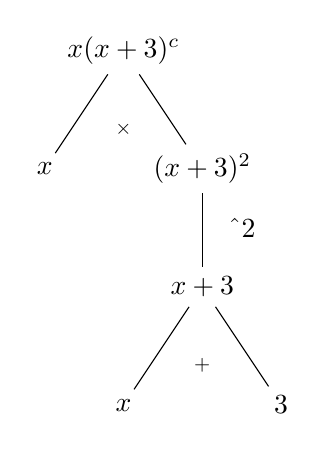
\begin{tikzpicture}[yscale=0.75]
        \node (f) at (0,0) {$x(x+3)^c$};
        \node[below of=f,scale=0.75] {$\times$};
        \node (x1) at (-1,-2) {$x$};
        \node (sqrt1) at (1,-2) {$(x+3)^{2}$}; 
        % \node[below of=sqrt1,scale=0.75] {$\circ$};
        \node (su) at (1.5,-3) {\textasciicircum 2};
        \node (u) at (1,-4) {$x+3$};
        \node (x2) at (0,-6) {$x$};
        \node[below of=u,scale=0.75] {$+$};
        \node (three) at (2,-6) {$3$};
        % \node (x3) at (0,-8) {$x$};
        % \node (x4) at (2,-8) {$x$};
        % \node[below of=x2,scale=0.75] {$\times$};

        \draw[-] (f) -- (x1);
        \draw[-] (f) -- (sqrt1);
        % \draw[-] (sqrt1) -- (su);
        \draw[-] (sqrt1) -- (u);
        \draw[-] (u) -- (x2);
        \draw[-] (u) -- (three);
        % \draw[-] (x2) -- (x3);
        % \draw[-] (x2) -- (x4);

    \end{tikzpicture}
\end{center}
Starting at the top, apply individualized 
rules for each step.  Substitute in a product $MN[x\defeq 7]$ you compute 
$M[x\defeq 7]N[x\defeq 7]$,
sometimes denoted by a ``leads to'' relation $\leadsto$. So,
with $M+N$ we can write,
\[
    (M+N)[x\defeq 7]\leadsto M[x\defeq 7]+N[x\defeq 7]
\]
At the end we finish off with rules like $3[x\defeq 7]\leadsto 3$ and $x[x\defeq 7]\leadsto 7$.
If we use $x\defeq 3$ or $x\defeq t$ we use the same procedure.

You may have been taught induction through stories of falling 
dominos.  Good.  But what if induction was more like climbing, 
and the domino illustration was bottling up the experience
of climbing stairs?  Surely its more fun to climb trees and mountains.
Climbing can go up (induct) or down (recurse).
So substitution was recursing, climbing down our tree to its roots, the constants 
and single variables where bases cases.  The branches had to be explored independently.

% Now do 
% $x\defeq c$, does this look right? 

\medskip
\noindent \textbf{Grammar.}
% Before diagnosing the problem, 
% Pause to appreciate how well this worked most
% of the time. 
Climbing could find many routes, even go in cirlces, but 
substitution happend upon a tree.  It is the
same thing you do when you diagram a sentence in grammar school, only with
English you can sometimes get cycles.  That we got a tree is owed to the fact
that the grammars for mathematics are basic and gentle, what Chompsky's 
\emph{Syntactic Structure} calls
\emph{context-free} grammars.\footnote{
    If an algebraist starts a talk with story that ``...It was thought  all natural 
    languages were context-free until some obscure dialect in the alps or Africa was found...'', 
    then tune out until they return to equations.  
    Linguist never had such illusions. Even English is not context-free, read  James Higginbotham.}  
How we worked through the tree is known as \emph{traversing}
the tree, but try to see it as just another induction/recursion metaphor.

To write down a context-free grammar we specify the atoms of our language.
For natural numbers we can used digits $0,1,\ldots, 9$.  Then we write down patterns of how to 
combine digits.  The separate cases are designated by the auxiliary symbol $|$ (which reads as ``or'').  Each rule 
is given an name called a \emph{token} (or \emph{tag}) and denoted \lstinline{<Name>}.
Since the Walrus $\defeq$ is our assignment of variables, we use the surprised Walrus $::=$ as assignment of token rules.
\begin{lstfloat}
\begin{lstlisting}[mathescape]
     <PosDig> ::= 1 | 2 | 3 | 4 | 5 | 6 | 7 | 8 | 9 
      <Digit> ::= 0 | <PosDig>
       <Nat>  ::= <Digit> | <PosDig><Nat>
\end{lstlisting}
\caption{The grammar for natural numbers.}
\end{lstfloat}

The natural number grammar is said to \emph{accept} $0$ as a digit, written ``0:Digit'' and also as 
a Nat, ``0:Nat''.  It also accepts 541:Nat and 10:Nat but it rejects ``01:Nat''
as that case does not exist as a rule for any token in this grammar.  Deciding to accept or 
reject is recursion, work down until you can decide.  Induction, which builds up, can only 
ever make strings that are in the grammar, so there is no question about accepting/rejecting 
by induction.


\begin{center}
\begin{tikzpicture}
    \node at (-3.5,0) {\begin{tikzpicture}
        \node (10) at (0,0) {10:Nat};
        \node (1) at (-2,-2) {1:PosDig};
        \node (0n) at ( 2,-2) {0:Nat};
        \node (0d) at ( 2,-4) {0:Digit};
        \draw[thick] (0d) -- (0n) -- (10) -- (1);
        \node[below of=10,scale=0.75,text width=0.6in] {Nat case 2};
        \node[scale=0.75,text width=0.6in] at ( 1.5,-3) {Nat case 1};
    \end{tikzpicture}};
    \node at (3.5,0) {\begin{tikzpicture}
        \node (01) at (0,0) {01:Nat};
        \node (1) at ( 2,-2) {1:PosDig};
        \node (0n) at (-2,-2) {0:Nat};
        \node (0d) at (-2,-4) {0:Digit};
        \draw[thick,dashed] (0n) -- (10) -- (1);
        \draw[thick] (0d) -- (0n);
        \node[below of=01,scale=0.75,text width=0.6in] {no case!};
        \node[scale=0.75,text width=0.6in] at (-1.3,-3) {Nat case 1};
    \end{tikzpicture}};
\end{tikzpicture}
\end{center}
The strings accepted by our grammar are known as the  \emph{language}
for that grammar.  

\medskip
\noindent\textbf{Operators.}
The rules in the grammar are often described as \emph{operators}.  For example,
\lstinline{<PosDig><Nat>} operates to take a positive digit and a natural number 
and form a new natural number.  We call it a \emph{binary} operator because it 
takes two inputs.  We also call it \emph{heterogeneous} because it takes in data 
of different types.  (If all the inputs and outputs are of the same type we call the operator 
\emph{homogeneous}.)  Some operators take in only one input, so called \emph{unary}, 
such as the first case of \lstinline{<Nat>} which takes in a digit and is said to \emph{promote} the 
term to a natural number.\footnote{Promote improves over the alternative \emph{coerce},
which in turn replaced the use of ``caste''---an all too casual allusions to a discriminator societal 
system.}
Operators that require no preexisting data, such 
as the digits $0,\ldots,9$, are called \emph{nullary}, or simply \emph{atomic}.

\begin{remark}
The symbols \lstinline{::=}, \lstinline{<Token>} and \lstinline{|} are 
Backus-Naur Form (BNF) notation, which is popular 
in computer science.  The idea under different notation was written 
down in 600 BC by Panini's rules of Sanskrit grammar.  Good ideas get rediscovered;
great ideas get stolen.
\end{remark}


\noindent\textbf{Multi-sorted grammars.} To add depth to this we add new sorts
of symbols.  The first sort are constants.  The next sort are variables, e.g.\
$x,y,x_0,x_1,\ldots$. A third sort can be operators, e.g.\ $+,-,\times,\div$.
To make things short lets drop down to the language of Boolean (true/false) algebra
instead.
\medskip

\noindent\textbf{Example.}
For Boolean (true/false) algebra we have true `$\top$', false `$\bot$', 
and `$\wedge$', or `$\vee$', and not `$\neg$' with the following grammar
which includes parenthesis. For example, $\top \vee (\neg(x_2\wedge y)\vee x_1):Bool$ but $Bool$ rejects $\bot\neg$.
\begin{lstfloat}[!hbtp]
\begin{lstlisting}[mathescape]
    <Var>  ::= x | y | x_<Nat> | y_<Nat>
    <Bool> ::= $\top$ 
             | $\bot$ 
             | <Var>
             | $\neg$ <Bool> 
             | <Bool> $\vee$ <Bool> 
             | <Bool> $\wedge$ <Bool>
             | (<Bool>)
\end{lstlisting}
\caption{A Boolean algebra grammar.}
\end{lstfloat}

There is something still missing.  Try reading $\neg(x_2\wedge y)\vee x_1$.  
Is this meant to negate $(x_2\wedge y)\vee x_1$ 
or is it to negate $(x_2\wedge y)$ and then or that with $x_1$? This grammar 
offers two associated parse trees.
\begin{center}
    \begin{tikzpicture}
        \node at (-3.5,0) {\begin{tikzpicture}
            \node (10) at (0,0) {$\neg(x_2\wedge y)\vee x_1:Bool$};
            \node (0n) at ( 0,-2) {$(x_2\wedge y)\vee x_1:Bool$};
            % \node (0d) at ( 2,-4) {0:Digit};
            \draw[thick] (0n) -- (10);
            % \node[below of=10,scale=0.75] {$\circ$};
            \node at (0.5,-1) {$\neg$};
            % \node[scale=0.75,text width=0.6in] at ( 1.5,-3) {Nat case 1};
        \end{tikzpicture}};
        \node at (3.5,0) {\begin{tikzpicture}
            \node (01) at (0,0) {$\neg(x_2\wedge y)\vee x_1:Bool$};
            \node (1) at (-2,-2) {$\neg(x_2\wedge y):Bool$};
            \node (0n) at ( 2,-2) {$x_1:Bool$};
            \draw[thick] (0n) -- (10) -- (1);
            \node[below of=01] {$\vee$};
        \end{tikzpicture}};
    \end{tikzpicture}
\end{center}
This is where \emph{order of operations} steps in to resolve the ambiguity.
One option is \emph{left-most outer-most (LeMOM)}, which---similar to English language,
reads from left to right and assumes we start to match the pattern from the 
outer most symbols.  So in $\neg(x_2\wedge y)\vee x_1$ the LeMOM
$\neg$ is the symbol we need to parse, which means it will ``parse'' once 
we succeed in forming a $Bool$.  So we move ahead and read 
$(x_2\wedge y)\vee x_1$.  Here the LeMOM is `(' which will need to match 
with \lstinline{<Bool>)}.  Reading further $x_2:Var$ which promotes to 
$x_2:Bool$, then $\wedge$ matches with $x_2:Bool\wedge y:Bool$
so that we have $x_2\wedge y:Bool$.  Then we hit `)' which matches 
our earlier `(' thus giving us $(x_2\vee y):Bool$ which finally matches with 
$\neg$\lstinline{<Bool>} and we parse $\neg(x_2\wedge y):Bool$.  At this point 
we have parsed $\neg$ and so we continue with $\vee$ to match 
$\neg(x_2\wedge y)\vee x_1:Bool$ with the right-hand-side parse tree.


LeMOM parsing is favored in mathematics and computer science because we can 
decide what things mean the moment we encounter them in the string.  
There are other orders of operations,
for example right-most inner-most (RiMIM) or the high-school PEMDAS
(Parenthesis, Exponential, Multiplication, Division, Addition, Subtraction). 
These allow for short formulas to be more expressive (jargon to mean they 
communicate more than a similarly long string in a less ``expressive'' language).
But parsing a grammar with such orders of operations is slower, often requiring 
us to read in everything before making even a single choice.  Take for example 
$(3x+9)^5$, it is the outermost exponent 5 that comes at the end which we will 
consider as the first step in parsing, i.e.\ the top of the tree.

\begin{quote}
\textbf{Grammar plus order of operations are a language to express a desired induction.}
\end{quote}

\noindent\textbf{Exercises}
\begin{enumerate}
    \item Write the grammar for decimal numbers.
    \item Write the grammar for a 4 function calculator with decimal numbers
    and $+,-,\times, \div$.
\end{enumerate}
\medskip
